%===============================Scientific Poster by C.Has================================
\documentclass[20pt]{beamer}

\usepackage[size=a0, orientation=portrait, scale=1.4]{beamerposter} 
\usetheme{Madrid}
\graphicspath{{Images/}}

\usepackage{changepage}
\usepackage{subcaption}
\usepackage{mathptmx}
\usepackage{booktabs}
\usepackage[numbers]{natbib}

\renewcommand{\raggedright}{\leftskip=0pt \rightskip=0pt}
\let\olditemize\itemize
\renewcommand{\itemize}{\olditemize\addtolength{\itemsep}{0.4\baselineskip}}

\addtobeamertemplate{block begin}{}{ \vspace{5mm}\begin{adjustwidth}{5mm}{5mm}}
\addtobeamertemplate{block end}{\end{adjustwidth}\vspace{10mm}}{ \vspace{5mm}}
\setbeamerfont{block title}{size={\centering\bfseries\fontsize{48}{60}\selectfont}}

\setbeamercolor{block body}{bg=white}
\setbeamercolor{background canvas}{bg=green!75}

\definecolor{title-color}{RGB}{127 96 0}
\setbeamercolor{chcolor}{fg=white, bg=title-color}

\setbeamertemplate{headline}{%
\begin{beamercolorbox}[wd=\paperwidth]{chcolor}\vskip5mm 
\begin{columns}
	\begin{column}{0.15\linewidth}
	\centering	
	
\includegraphics[width=0.85\linewidth]{logo}	 
	\end{column}
 
	 \begin{column}{0.85\linewidth}
	\centering\bfseries 	
	{\fontsize{80}{96}\selectfont How to Create Scientific Poster in \LaTeX} \\[6mm]
	{\fontsize{60}{72}\selectfont \underline{Author A}, Author B, and Author C$^\star$}\\[6mm]
	{\fontsize{48}{60}\selectfont Department of Chemical Engineering, Indian Institute of Technology Bombay}\\[3mm]
	{\fontsize{48}{60}\selectfont Mumbai, Powai-400076}\\[6mm] 
	{\fontsize{36}{42}\selectfont $^\star$Email: authorC@email.com}	
	\end{column}
\end{columns}\vskip5mm	
\end{beamercolorbox}
%
\color{red}\rule{\paperwidth}{20pt}

} 

\setbeamercolor{chfootcolor}{fg=white, bg=black}
\setbeamertemplate{footline}{%
\begin{beamercolorbox}[wd=\paperwidth, center, ht=1.5em]{chfootcolor}
\small	For any suggestions/queries: authorA@email.com
\end{beamercolorbox}
}
 
 %========================================Document body==============
\begin{document}\vspace*{-2cm}
\begin{frame}[t]
\begin{columns}[t]

%=================================col-1============================	
\begin{column}{0.32\linewidth}
\begin{block}{Introduction}
LaTeX, which is pronounced Lah-tech or Lay-tech, is
a document preparation system for high-quality type-
setting. It is most often used for medium to large
technical or scientific documents but it can be used
for almost any form of publishing.

\begin{itemize}
	\item Posters are a great way to showcase your work,
	whether at conferences, class presentations, or
	university open days.
	
	\item Conference posters are used by researchers to dis-
	play the results of research at academic confer-
	ences.
	
	\item They are printed on large paper (typically A0) and
	use large font sizes to rapidly draw attention.
	Typically, a number of sections are present to
	summarize the background, experimental design,
	results and significance of the experiment per-
	formed as succinctly as possible.
	
	\item Text is therefore best kept to a minimum and
	results are shown visually in tables, figures and
	equations.
	
	\item LaTeX makes creating posters as easy as writing
	a normal document and can be customized to
	create beautiful poster layouts.	
\end{itemize}

\vskip2cm 

\begin{figure}
	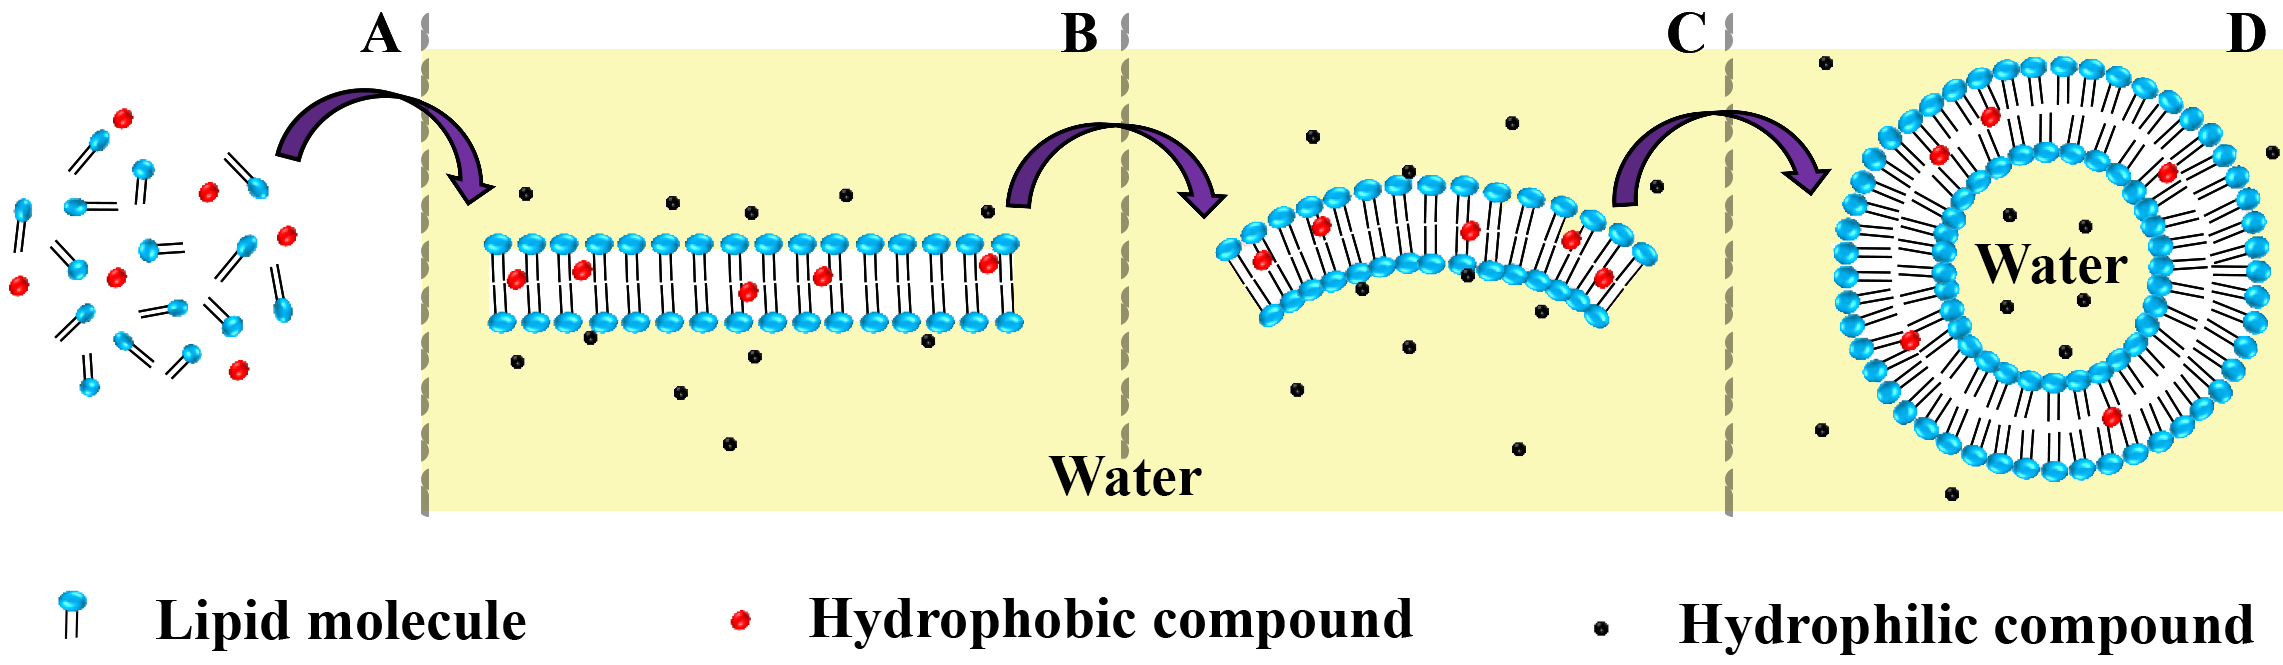
\includegraphics[width=\linewidth]{intro}
	\caption{This is an example of adding an image poster~\cite{hasc18,has2019comprehensive}.}
\end{figure}	
\end{block}		
%--------------------------
	
\begin{block}{Background and Motivation}
\begin{itemize}
\item Lorem Ipsum is simply dummy text of the printing
 and typesetting industry.

\item Lorem Ipsum has been the industry’s standard
 dummy text ever since the 1500s, when an un-
 known printer took a galley of type and scrambled
 it to make a type specimen book.

\item It has survived not only five centuries, but also the
 leap into electronic typesetting, remaining essen-
 tially unchanged.
\end{itemize}

\vskip2cm 

\begin{figure}
	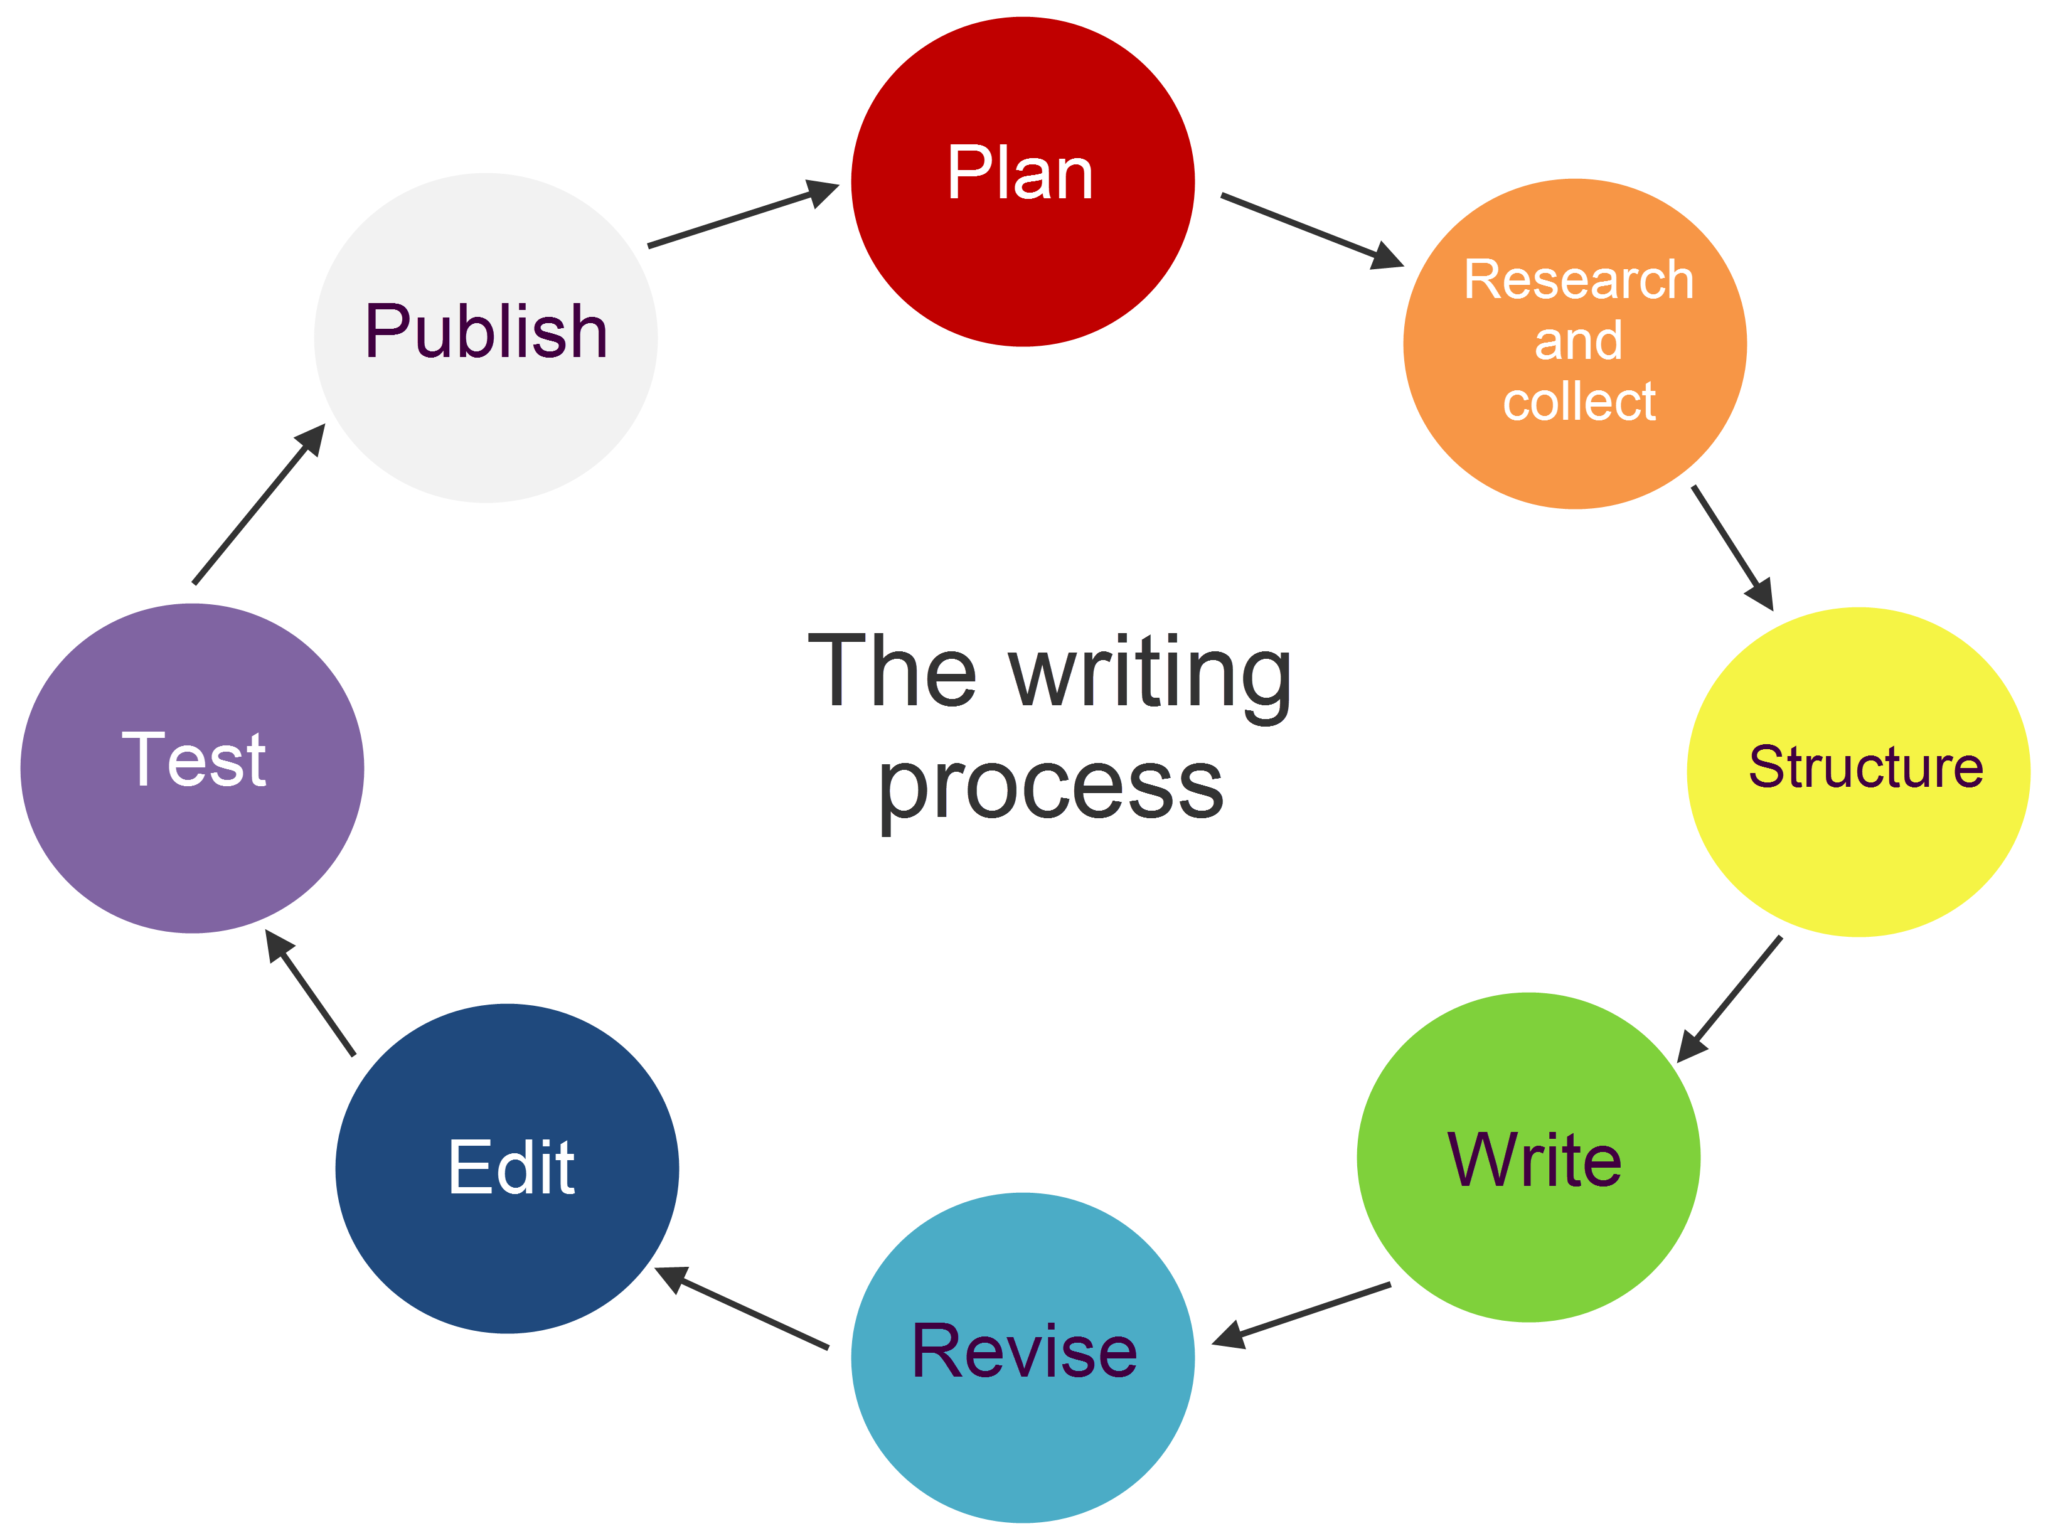
\includegraphics[width=\linewidth]{wp}
	\caption{The common steps involved in writing process.}
\end{figure}	

\vspace{12.5cm}	
\end{block}		
\end{column}		

%====================================col-2========================
\begin{column}{0.32\linewidth}
	\begin{block}{Materials and Methods}
	\textbf{\underline{Materials}}	

\begin{itemize}
	\item There are many variations of passages of Lorem
	Ipsum available, but the majority have suffered
	alteration in some form, by injected humour, or
	randomised words which don’t look even slightly
	believable.
	
	\item If you are going to use a passage of Lorem Ipsum,
	you need to be sure there isn’t anything embar-
	rassing hidden in the middle of text.
	
	\item In a free hour, when our power of choice is un-
	trammelled and when nothing prevents our being
	able to do what we like best, every pleasure is to
	be welcomed and every pain avoided.
\end{itemize}	

\textbf{\underline{Methods}}

\vspace{1cm}

\begin{figure} 	 
	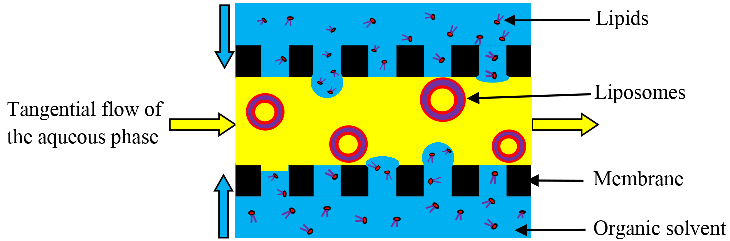
\includegraphics[width=0.95\linewidth]{setup}
	\caption{The experimental setup~\cite{jaafar2011new}.}	
\end{figure}

\begin{itemize}
	\item Lipid-ethanol solution is first heated at $T>T_g$ ,
	The fluid is conveyed through a tube to the module.
	
	\item In module, it is extruded through a membrane
	contactor with definite pore size.
	
	\item Simultaneously, the aqueous solution is tangen-
	tially flowed on the membrane contactor.
\end{itemize}

\vspace{1cm}

Bond interaction between two atoms A and B can be represented by the following potential energy functional:
\begin{equation*}
E=U(r_\mathrm{AB}= 1/2\kappa_\mathrm{AB}(r_\mathrm{AB}-r_\mathrm{AB,eq})^2
\end{equation*}
	\end{block}	
	
\begin{block}{Results}
\vspace{1cm}
	
\begin{minipage}[t]{0.4\linewidth}
	\begin{figure}
		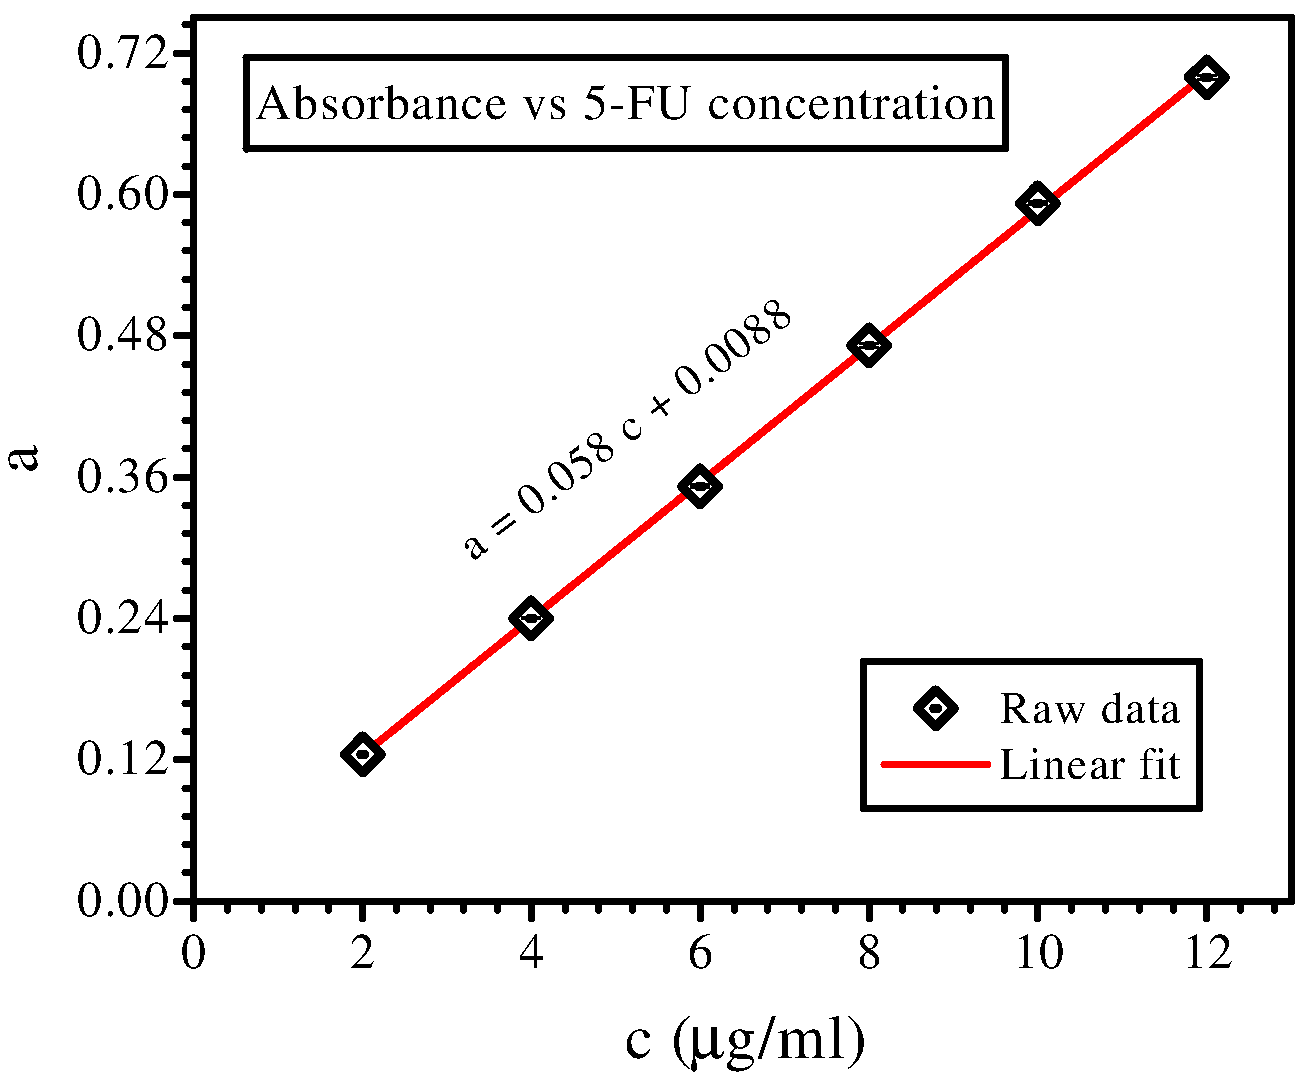
\includegraphics[width=\linewidth]{res1}
		\caption{5-FU calibration plot~\cite{hasc18}.}
	\end{figure} 
\end{minipage} 
~
\begin{minipage}[t]{0.35\linewidth}
	\begin{itemize}
		\item Note 1
		\item Note 2
		\item Note 3	
	\end{itemize}
\end{minipage} 		

\vspace{1cm}

\begin{figure}
	\begin{subfigure}[b]{0.45\linewidth}
		\centering		 
		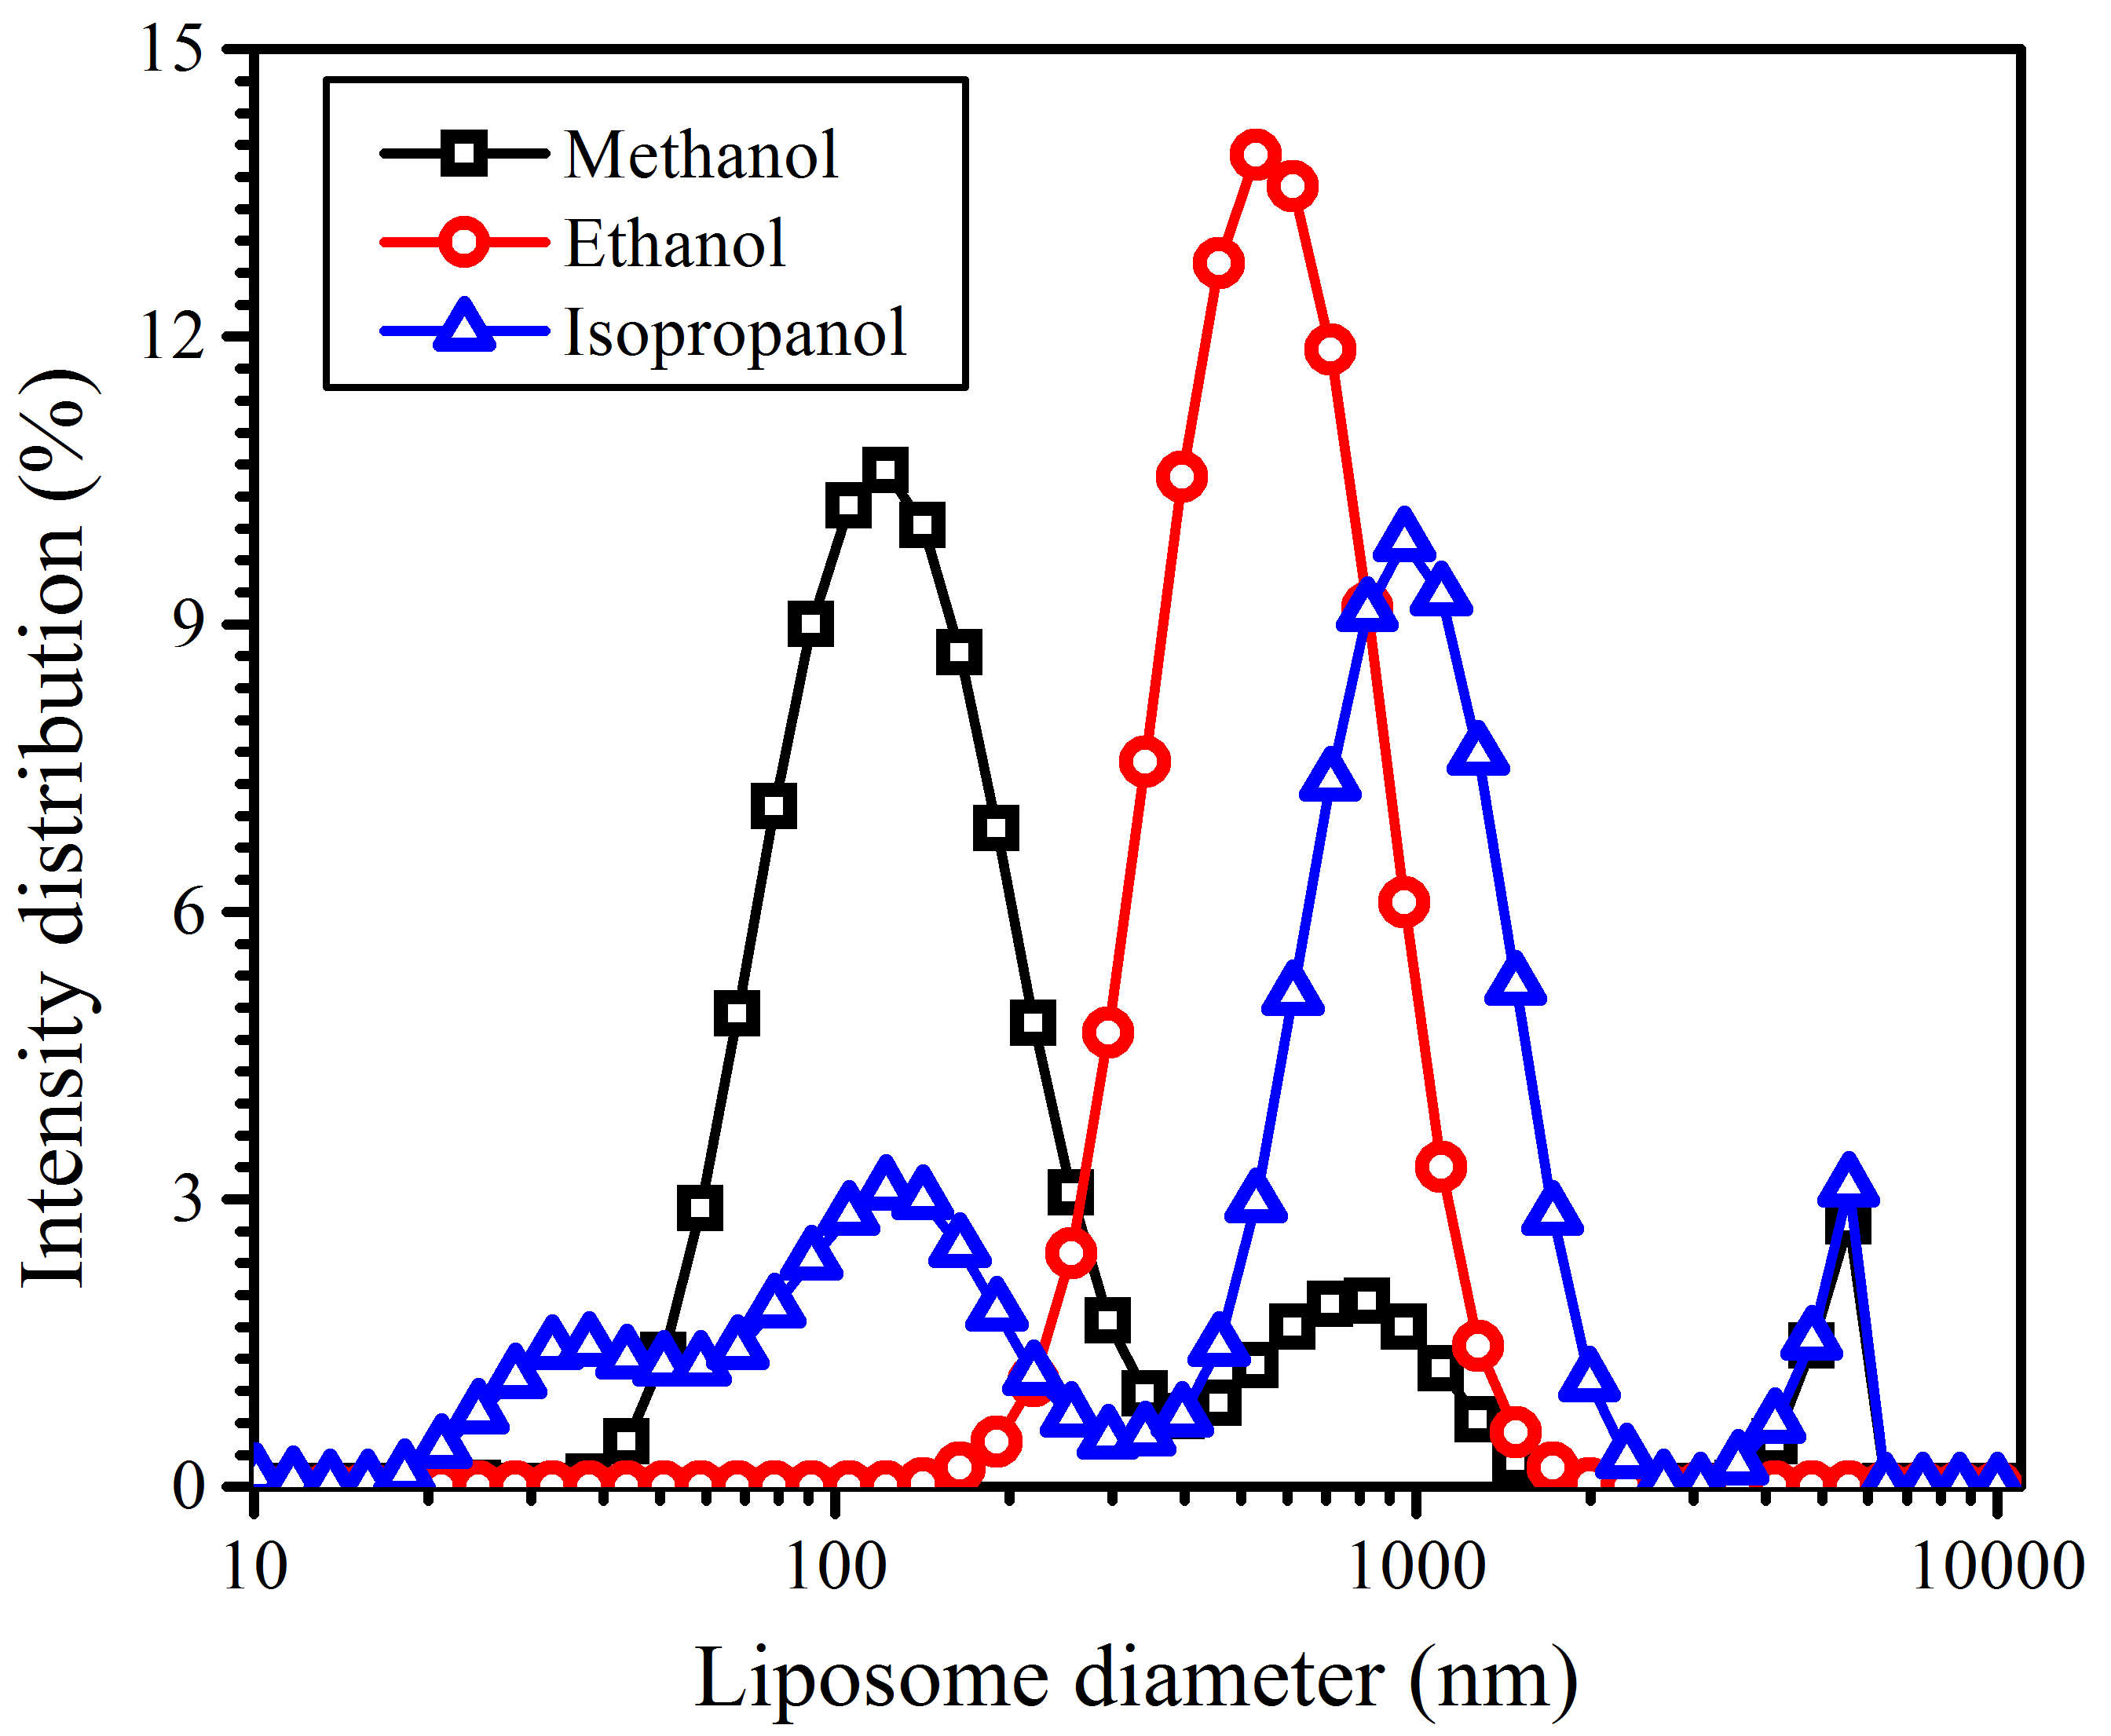
\includegraphics[width=0.9\linewidth]{res2}
		\caption{}	
	\end{subfigure} 
	~
	\begin{subfigure}[b]{0.45\linewidth}	
		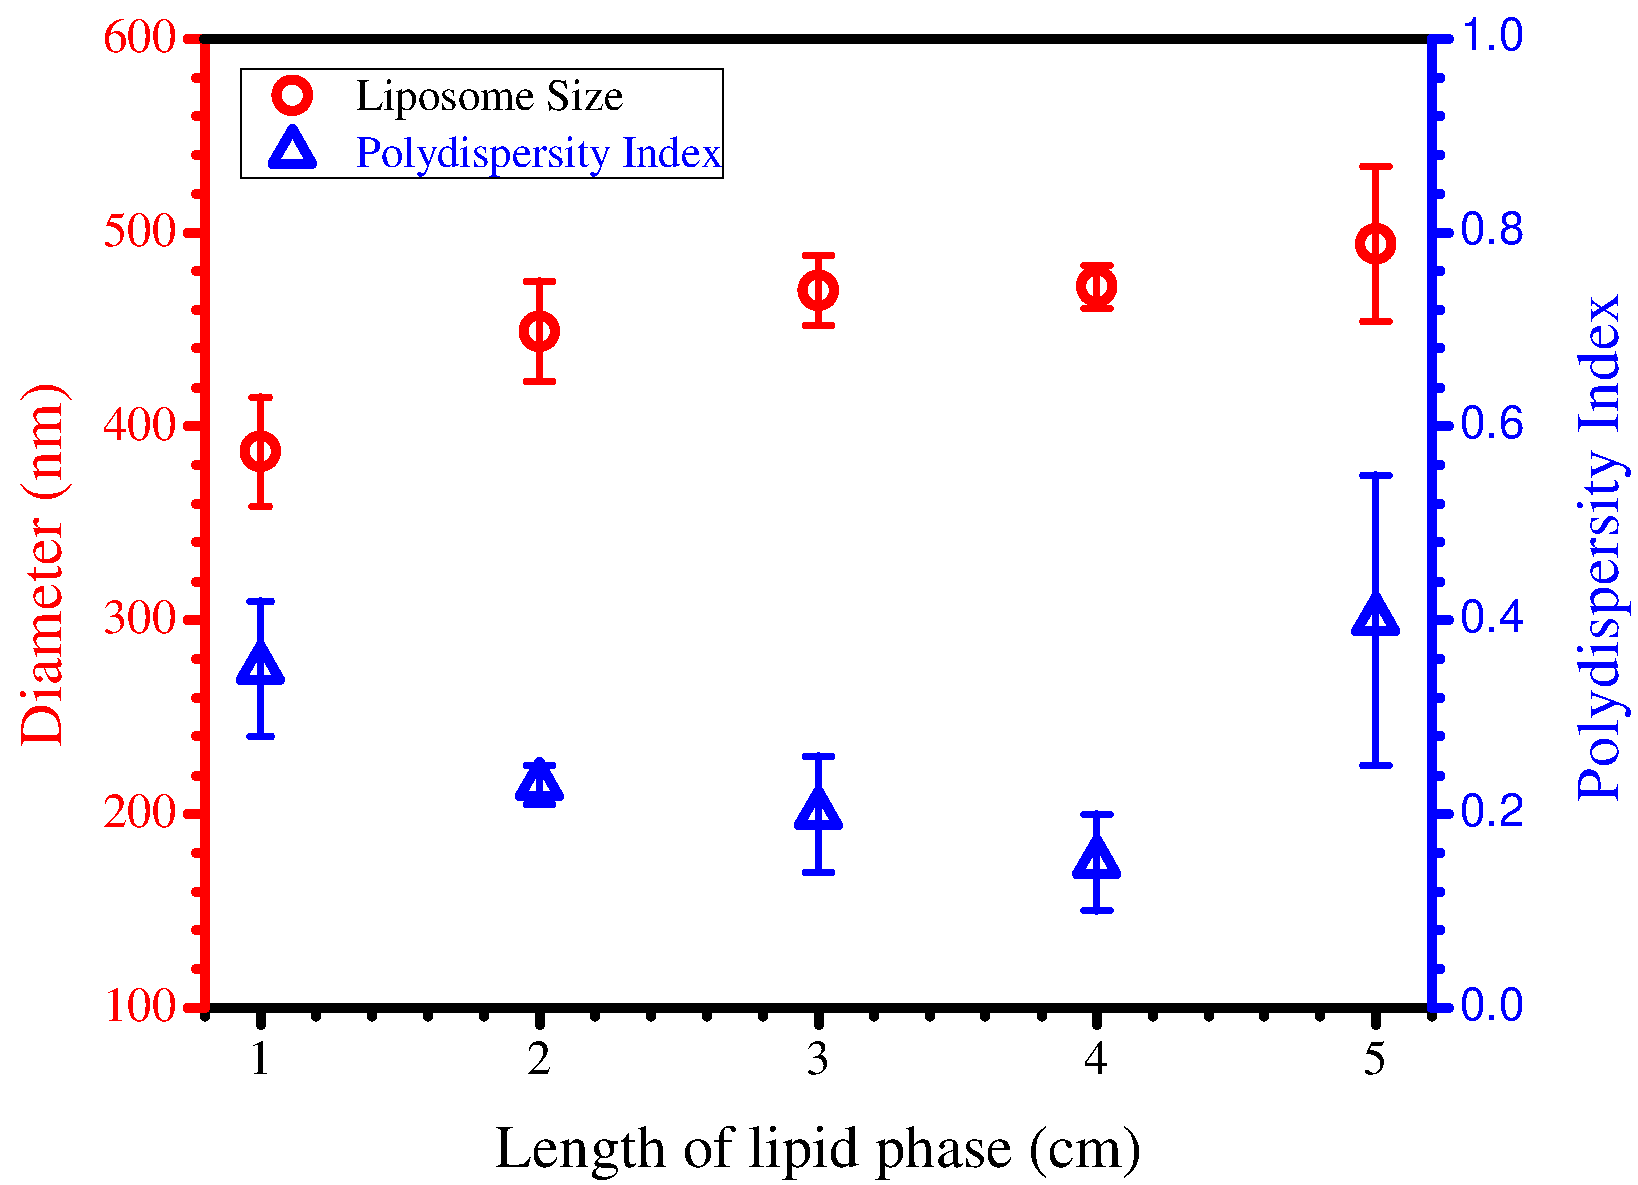
\includegraphics[width=\linewidth]{res3}
		\caption{}	    
	\end{subfigure} 
	\caption{This is an example of adding subfigures in latex~\cite{has2018rapid}.}
\end{figure} 

\vspace{1cm}

\begin{figure}
	
\includegraphics[width=0.65\linewidth]{res4}
	\caption{Mechanical response of adherent giant liposomes~\cite{sorkin2018nanomechanics}.}
\end{figure}

\vspace{3.7cm} 
\end{block}		 
\end{column}	

%=================================col-3============================	
\begin{column}{0.32\linewidth}	
\begin{block}{Results}

\textbf{\underline{Comparison of different proposed methods}}

\vspace{1cm}

\begin{figure}
	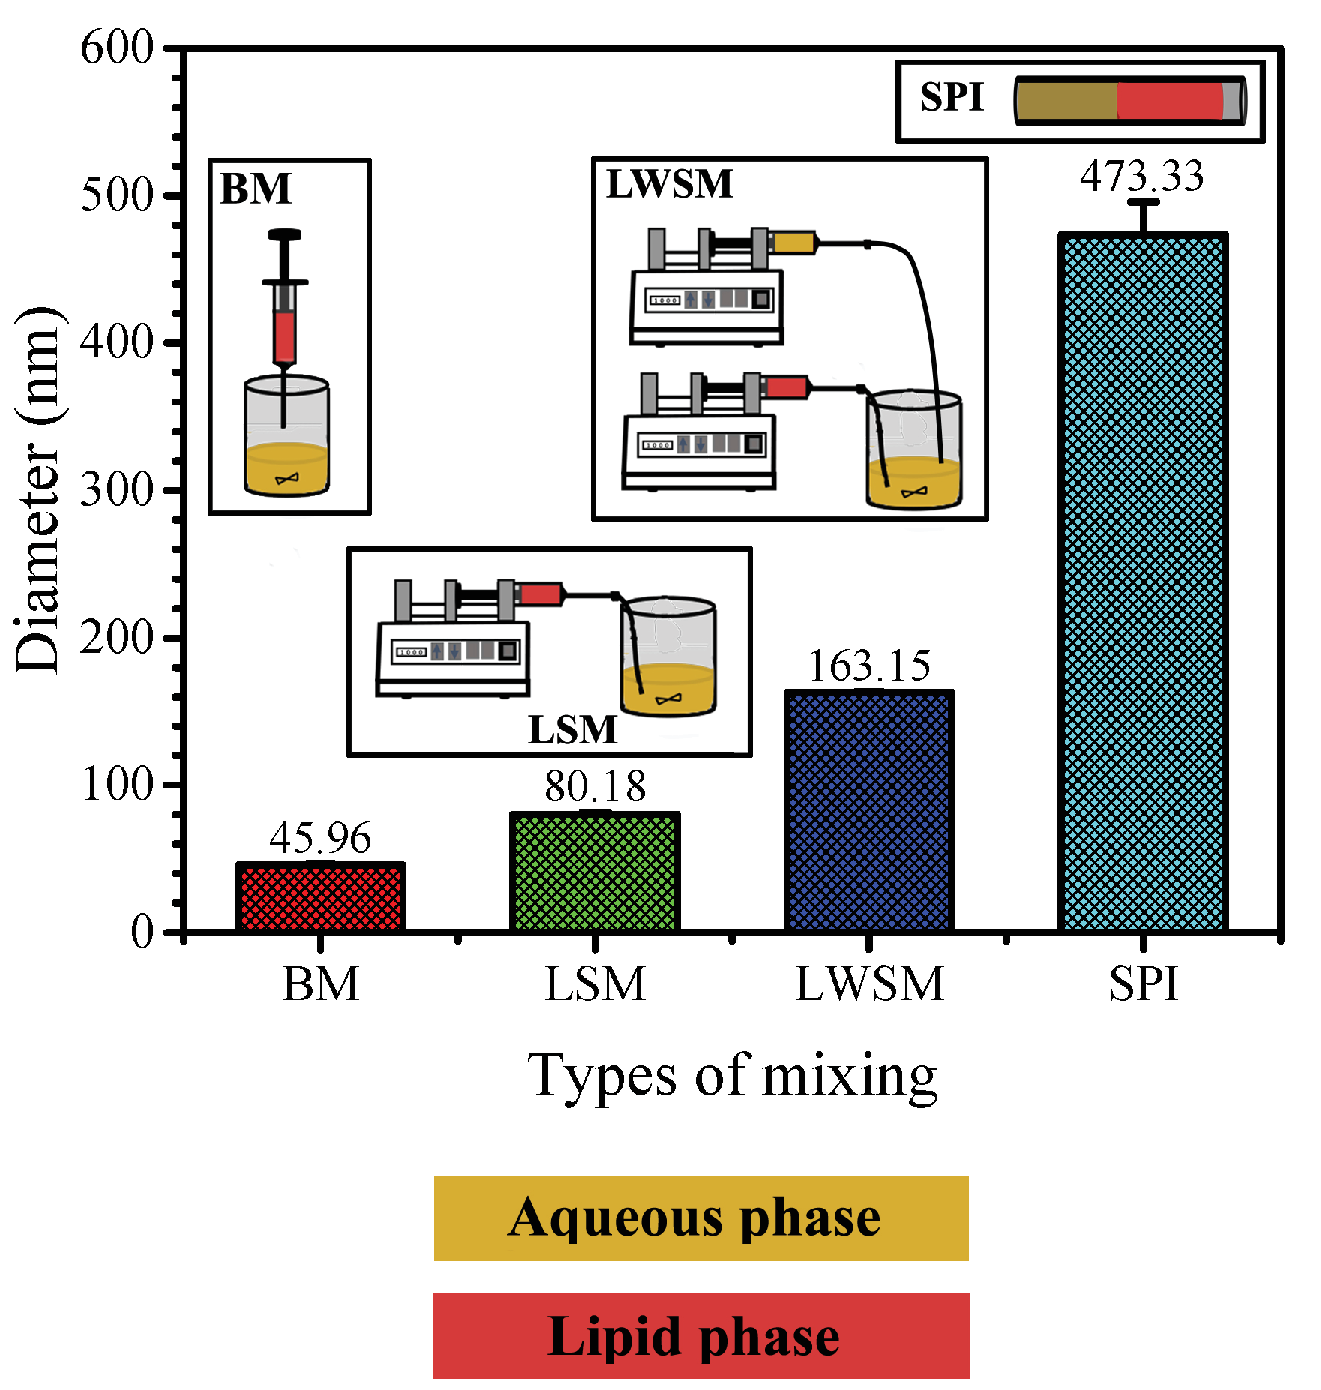
\includegraphics[width=0.74\linewidth]{res5}
	\caption{Mechanical response of adherent giant liposomes~\cite{sorkin2018nanomechanics}.}
\end{figure}  	

\vspace{1cm}

\begin{table}\small 
	\begin{tabular}{llll}	
		\toprule
		Method & Step & Lamellarity &  Size (nm) \\
		\midrule
		TFH & Multi & Multilamellar & MLVs \\
		DD & Multi & Unilamellar & LUVs \\
		REV & Multi & Multilamellar & LUVs, OLVs\\
		EI & Single & Unilamellar & SUVs, LUVs \\
		ED & Multi & Unilamellar & GUVs \\
		PS & Single &  Unilamellar & SUVs, LUVs, GUVs \\
		\bottomrule
	\end{tabular}	
\end{table}	
	
\end{block}		

\begin{block}{Conclusions}
\begin{itemize}
	\item  Lorem Ipsum is simply dummy text of the printing and typesetting industry.
	
	\item   It was popularised in the 1960s with the release of Letraset sheets containing Lorem Ipsum passages, and more recently with desktop publishing software like Aldus PageMaker including versions of Lorem Ipsum.
	
	\item  It is a long established fact that a reader will be distracted by the readable content of a page when looking at its layout. 
	
	\item  Various versions have evolved over the years, sometimes by accident, sometimes on purpose (injected humour and the like).
	
	\item No one rejects, dislikes, or avoids pleasure itself, because it is pleasure, but because those who do not know how to pursue pleasure rationally encounter consequences that are extremely painful. 
	
	\item Lorem Ipsum is simply dummy text of the printing and typesetting industry.	
\end{itemize}		
\end{block}	

\begin{block}{References}
\bibliography{mybib}
\bibliographystyle{rsc}	
	
\end{block}	

\begin{block}{Acknowledgements}
Lorem ipsum dolor sit amet, consectetur adipiscing
elit, sed do eiusmod tempor incididunt ut labore et
dolore magna aliqua. Ut enim ad minim veniam, quis
nostrud exercitation ullamco laboris nisi ut aliquip ex
ea commodo consequat.	

\vspace{1.5cm}	
\end{block}		
\end{column}	
		
\end{columns}	  
\end{frame}
\end{document}
%========================================================================= 